\documentclass{article}
\usepackage[english,russian]{babel}
\usepackage{textcomp}
\usepackage{geometry}
  \geometry{left=2cm}
  \geometry{right=1.5cm}
  \geometry{top=1.5cm}
  \geometry{bottom=2cm}
\usepackage{tikz}
\usepackage{multicol}
\usepackage{listings}
\pagenumbering{gobble}

\lstdefinestyle{csMiptCppStyle}{
  language=C++,
  basicstyle=\linespread{1.1}\ttfamily,
  columns=fixed,
  fontadjust=true,
  basewidth=0.5em,
  keywordstyle=\color{blue}\bfseries,
  commentstyle=\color{gray},
  texcl=true,
  stringstyle=\ttfamily\color{orange!50!black},
  showstringspaces=false,
  %numbers=false,
  numbersep=5pt,
  numberstyle=\tiny\color{black},
  numberfirstline=true,
  stepnumber=1,      
  numbersep=10pt,
  backgroundcolor=\color{white},
  showstringspaces=false,
  captionpos=b,
  breaklines=true
  breakatwhitespace=true,
  xleftmargin=.2in,
  extendedchars=\true,
  keepspaces = true,
  tabsize=4,
  upquote=true,
  emph = {override, final},
  emphstyle={\color{blue}\bfseries},
}
\lstdefinestyle{csMiptCppBorderStyle}{
  style=csMiptCppStyle,
  framexleftmargin=5mm, 
  frame=shadowbox, 
  rulesepcolor=\color{gray}
}

\lstset{style=csMiptCppStyle}
\lstset{literate={~}{{\raisebox{0.5ex}{\texttildelow}}}{1}}


\begin{document}
\title{Семинар \#2: Полиморфизм \vspace{-5ex}}\date{}\maketitle

\section*{Полиморфизм}
\textbf{Полиморфизм} -- это способность функций обрабатывать данные разных типов.
\subsection*{Статический полиморфизм}
\subsection*{Динамический полиморфизм}


\section*{Виртуальные функции}
Виртуальные функции (также известные как виртуальные методы) -- это механизм, который позволяет осуществлять полиморфизм.
Виртуальные функции позволяют динамически определять, какая функция будет вызвана в зависимости от типа объекта, а не типа указателя или ссылки, указывающего на этот объект.

Чтобы указать, что какой-либо метод является виртуальным, нужно использовать ключевое слово \texttt{virtual} в объявлении метода в базовом классе. После этого этот метод, а также все методы с такой же сигнатурой во всех производных классах станут виртуальными. Использовать \texttt{virtual} в объявлениях методов производных классов необязательно. Виртуальный метод отличается от обычного следующим:

\begin{center}
\textit{Если в программе возникнет ситуация когда указатель (или ссылка) на базовый класс будет указывать на объект производного класса, то при вызове виртуального метода через этот указатель (или ссылку) будет вызываться метод производного класса, а не метод базового класса.}
\end{center}


\subsection*{Объект базового класса, инициализированный объектом производного}
\begin{multicols}{2}
\begin{lstlisting}[style=csMiptCppBorderStyle]
#include <iostream>
struct Alice 
{
    void say() 
    {
    	std::cout << "Alice" << std::endl;
    }
};

struct Bob : public Alice 
{
    void say() 
    {
    	std::cout << "Bob" << std::endl;
    }
};

int main() 
{
    Bob b;
	Alice a = b;
    a.say();  // Напечатает Alice
}
\end{lstlisting}


\begin{lstlisting}[style=csMiptCppBorderStyle]
#include <iostream>
struct Alice 
{
    virtual void say() 
    {
    	std::cout << "Alice" << std::endl;
    }
};

struct Bob : public Alice 
{
    void say() 
    {
    	std::cout << "Bob" << std::endl;
    }
};

int main() 
{
    Bob b;
	Alice a = b;
    a.say();  // Всё равно напечатает Alice
}
\end{lstlisting}
\end{multicols}

\subsection*{Указатели на базовый класс, хранящие адрес объекта производного класса}
Виртуальные функции работают в случае когда есть указатель (или ссылка) на базовый класс, который указывает на объект производного класса. 
\begin{multicols}{2}\noindent
\begin{lstlisting}[style=csMiptCppBorderStyle]
#include <iostream>
struct Alice 
{
    void say() 
    {
    	std::cout << "Alice" << std::endl;
    }
};

struct Bob : public Alice 
{
    void say() 
    {
    	std::cout << "Bob" << std::endl;
    }
};

int main() 
{
    Bob b;
	Alice* pa = &b;
    a->say();  // Напечатает Alice
}
\end{lstlisting}


\begin{lstlisting}[style=csMiptCppBorderStyle]
#include <iostream>
struct Alice 
{
    virtual void say() 
    {
    	std::cout << "Alice" << std::endl;
    }
};

struct Bob : public Alice 
{
    void say() 
    {
    	std::cout << "Bob" << std::endl;
    }
};

int main() 
{
    Bob b;
	Alice* pa = &b;
    a->say();  // Напечатает Bob
}
\end{lstlisting}
\end{multicols}

\newpage
\subsection*{Вызов виртуальных функций из методов класса}
Ещё один случай когда работают виртуальные функции -- если мы вызываем виртуальный метод из другого метода (не важно виртуального или не виртуального).

\begin{multicols}{2}\noindent
\begin{lstlisting}[style=csMiptCppBorderStyle]
#include <iostream>
struct Alice 
{
    void say() 
    {
    	std::cout << "Alice" << std::endl;
    }    
    
    void func() 
    {
    	say();
    }
};

struct Bob : public Alice 
{
    void say() 
    {
    	std::cout << "Bob" << std::endl;
    }
};

int main() 
{
    Bob b;
	b.func();  // Напечатает Alice
}
\end{lstlisting}


\begin{lstlisting}[style=csMiptCppBorderStyle]
#include <iostream>
struct Alice 
{
    virtual void say() 
    {
    	std::cout << "Alice" << std::endl;
    }    
    
    void func() 
    {
    	say();
    }
};

struct Bob : public Alice 
{
    void say() 
    {
    	std::cout << "Bob" << std::endl;
    }
};

int main() 
{
    Bob b;
	b.func();  // Напечатает Bob
}
\end{lstlisting}
\end{multicols}

\newpage
\subsection*{Виртуальные функции в конструкторах и деструкторах}
Если производный класс вызывает конструктор базового класса (это происходит автоматически в перед вызовом конструктора производного класса) и в конструкторе базового класса вызывается виртуальный метод, то вызовется метод базового класса.
Это происходит просто потому что объект производного класса не может вызывать свои методы, так как он ещё не готов к этому. 
\begin{lstlisting}[style=csMiptCppBorderStyle]
#include <iostream>
struct Alice 
{
    Alice()     {say();}
    void func() {say();}
    virtual void say() 
    {
    	std::cout << "Alice" << std::endl;
    }
};

struct Bob : public Alice 
{
    void say() 
    {
    	std::cout << "Bob" << std::endl;
    }
};

int main() 
{
    Bob b;     // Напечатает Alice
    b.func();  // Напечатает Bob
}
\end{lstlisting}
Похожая ситуация будет и при вызове виртуального метода в деструкторе:
\begin{lstlisting}[style=csMiptCppBorderStyle]
#include <iostream>
struct Alice 
{
    virtual void say() {std::cout << "Alice" << std::endl;}
    void func() {say();}
    virtual ~Alice()    {say();}
};

struct Bob : public Alice 
{
    void say() {std::cout << "Bob" << std::endl;};
    ~Bob() {}
};

int main() 
{
    Bob b;
    b.func();  // Напечатает Bob
               // Напечатает Alice при уничтожении объекта
}
\end{lstlisting}



\subsection*{Виртуальный деструктор}

\subsection*{\texttt{override} и \texttt{final}}

\subsection*{Полиморфизм и умные указатели}

\subsection*{Как программа понимает, какой виртуальный метод вызывать}
Размер объектов полиморфных типов. Скрытый указатель на таблицу виртуальных функций.


\section*{Абстрактные функции}
\subsection*{Чистые виртуальные функции}
\subsection*{Абстрактные классы и интерфейсы}
\subsection*{Контейнер указателей на базовый класс, хранящих адрес объектов производных классов}
\subsection*{pure virtual call и определение чистых виртуальных методов}




\section*{RTTI и \texttt{dynamic\_cast}}
\subsection*{Полиморфный тип}
\subsection*{\texttt{dynamic\_cast}}

\subsubsection*{\texttt{dynamic\_cast} от родителя к ребёнку}
\subsubsection*{\texttt{dynamic\_cast} в бок}

\subsection*{Оператор \texttt{typeid} и класс \texttt{std::type\_info}}




\newpage
\section*{Реализация механизма виртуальных функций}
\begin{lstlisting}[style=csMiptCppBorderStyle]
#include <iostream>
struct Alice 
{
    virtual void say() 
    {
    	std::cout << "Alice Say" << std::endl;
    }
    virtual void walk() 
    {
    	std::cout << "Alice Walk" << std::endl;
    }
};

struct Bob : public Alice 
{
    virtual void say() 
    {
    	std::cout << "Bob Say" << std::endl;
    }
    virtual void walk() 
    {
    	std::cout << "Bob Walk" << std::endl;
    }
};

int main() 
{
    Alice a;
    Bob b;
    
    Alice* p = &a;
    p->say();  // Напечатает Alice Say
    
    p = &b;
    p->say();  // Напечатает Bob Say
}
\end{lstlisting}
\begin{center}
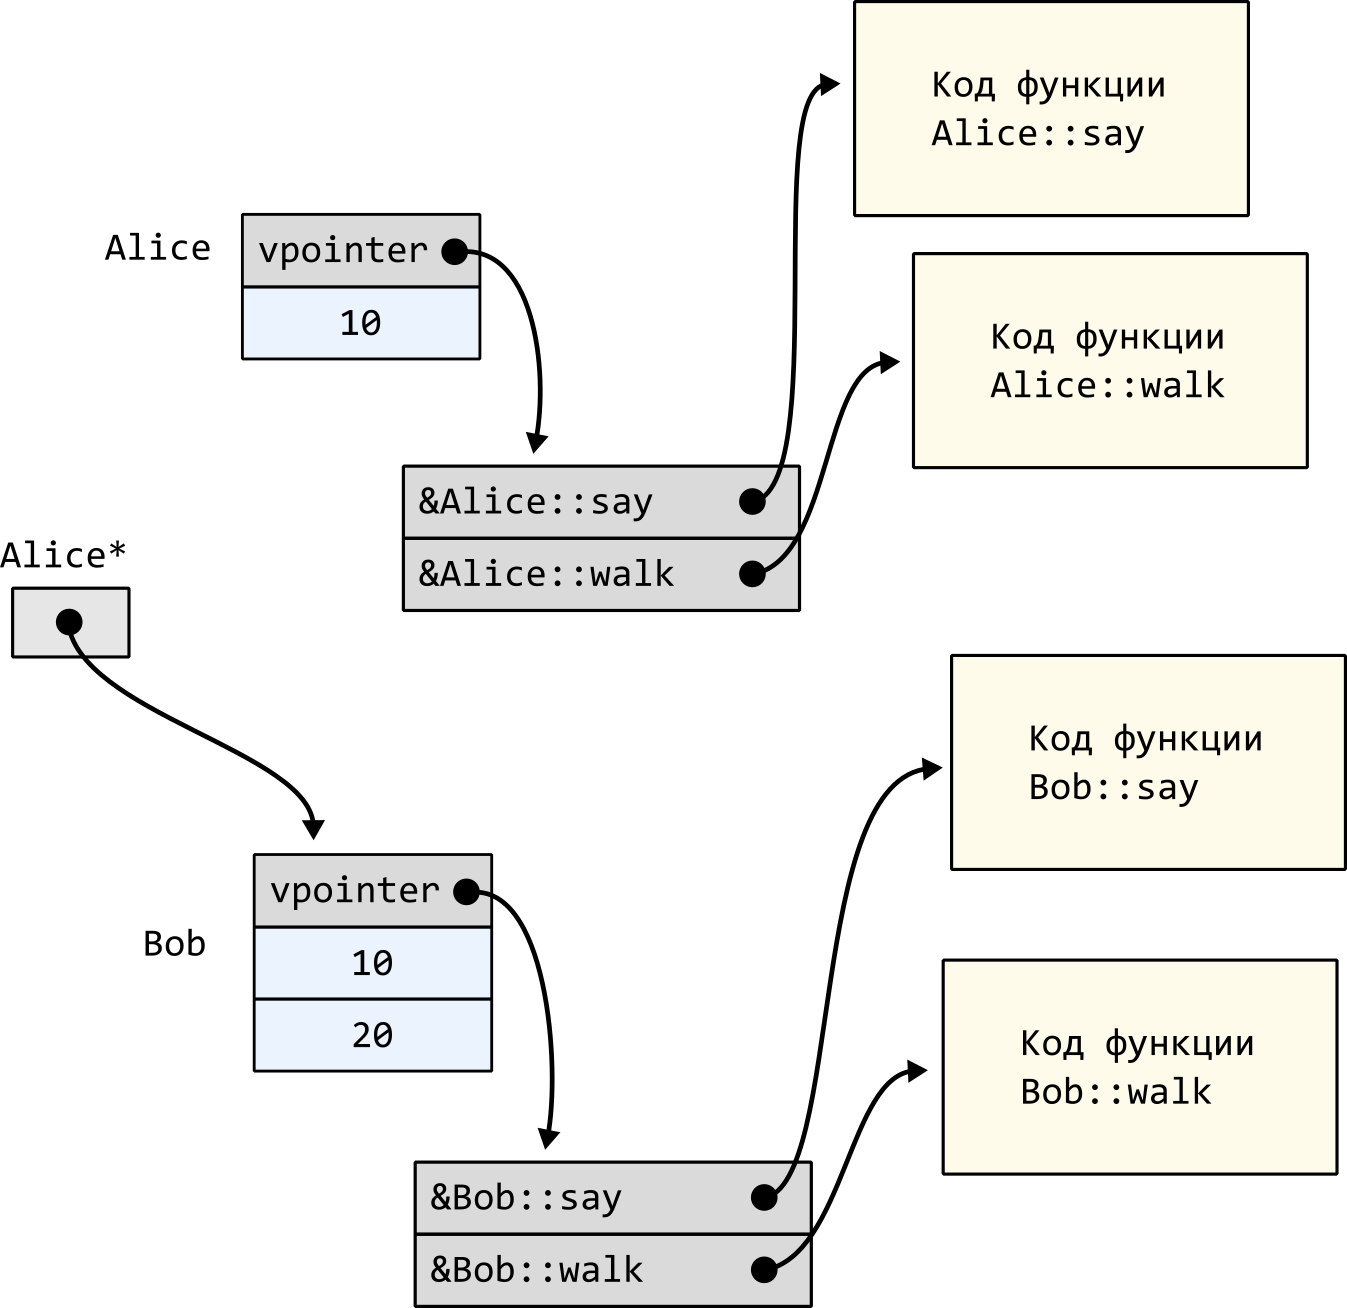
\includegraphics[scale=0.9]{../images/virtual_table_alice_bob.png}
\end{center}

\end{document}
